\chapter{Analyzing Existing Recommendation Systems}
\label{chap-suggs}

\Framework is a framework to create automated recommendations improving how developers perceive and respond to suggestions by incorporating \textbf{\em actionability}, \textbf{\em feedback}, and \textbf{\em locality}. The preliminary evaluation of this framework shows developers prefer actionable recommendations, however each principle factors into recommendations to developers and their overall impact on developer behavior remains unknown. To evaluate this approach, I first analyze the framework within existing recommender systems. This chapter explains how \suggs adheres to the \framework principles and presents two studies analyzing \sugg to explore their impact on the style and impact of recommendations. Additional study materials for these evaluations are available in Appendix~\ref{app-suggs}.

\section{GitHub \textit{Suggested Changes}}
\label{sec-suggs}

GitHub, a popular online code hosting site with millions of developers and billions of code contributions each year~\cite{Octoverse}, introduced the \textsl{suggested changes} feature as a public beta release in October 2018. Since the announcement, the GitHub blog reports users have been ``quick to adopt suggested changes'' into their code review processes with over 100,000 uses within weeks of the initial public beta release, accounting for 4\% of pull request comments and 10\% of code reviewers during that time~\cite{SuggestedChanges2}. This system, illustrated in Figure~\ref{fig:suggs}a-c, allows developers to make recommendations for code improvements to peers on GitHub during pull request reviews. The work presented in this chapter is the first research, to my knowledge, to study the \suggs feature.

To use the \suggs feature, a reviewer observes a deficient line of code on a pull request, they can click on the plus (+) sign on the line of code in question, in this case Line 9, to generate a pull request review comment (Figure~\ref{fig:suggs}a). Then, a text box is displayed for reviewers to enter a comment and they can click the \suggs icon (\includegraphics[height=1em]{Chapter-5/images/sugg_icon.png}) to propose changes to the line of code. Figure \ref{fig:suggs}b presents an example recommendation, where the reviewer encourages the developer not to use a single character variable name, which is discouraged in the Java programming language for non-temporary variables,\footnote{\url{https://www.oracle.com/java/technologies/javase/codeconventions-namingconventions.html}}, and recommends changing the variable name from \texttt{int c} to a more descriptive identifier \texttt{int count}. Once the reviewer finishes their suggestion, they can click on the ``Start a review'' button to submit their recommendation. Finally, the developer who submitted the pull request can see the suggested change on their code, shown in Figure \ref{fig:suggs}c, and has the ability to commit, edit, or ignore the proposed modification. Clicking on ``Commit changes'' provides the ability to automatically incorporate the proposed change into the pull request as a new commit.

\suggs can also be considered a nudge, encouraging developers to improve their code without providing incentives to apply reviewer suggestions (i.e. money) and allowing alternative changes to improve the code (i.e. \texttt{int compute}). Additionally, this system incorporates all of the developer recommendation choice architectures presented in Chapter~\ref{chap-framework}: it is \textit{actionable} by providing the ability for developers to automatically apply recommendations from peers by clicking on a button to commit suggestions (Figure~\ref{fig:suggs}c); provides informative \textit{feedback} to users by providing a specific improvement to the code with an optional comment (Figure~\ref{fig:suggs}b); has convenient \textit{locality} with recommendations appearing to developers on the exact line of code within their pull request and during code reviews before contributions are merged into the code (Figure~\ref{fig:suggs}a). By evaluating the design of this novel feature, I aim to explore the impact of \framework on recommendations to developers within this system and provide implications for designing of future recommender bots.

\begin{figure*}[htbp]
\centering
\subfloat[New suggested changes feature on GitHub pull requests]{\includegraphics[width=0.9\linewidth]{Chapter-5/images/sugg1.png}}\\
\centering
\subfloat[Reviewer adds comment and suggested change to modified line of code~]{\includegraphics[width=0.9\linewidth]{Chapter-5/images/sugg2.png}}\\
\subfloat[Developer can apply suggested change and commit to PR]{\includegraphics[width=0.9\linewidth]{Chapter-5/images/sugg3.png}}
\caption{Example of the \suggs feature}
\label{fig:suggs}
\end{figure*}



\section{Recommendation Styles}

\textit{Recommendation styles} refers to techniques utilized by automated approaches for conveying developer behavior recommendations to programmers. Prior work suggests styles of suggestions can impact the decision-making and behavior of users. For example, Fischer argues active help systems that automatically provide help to users are more effective than passive approaches~\cite{Fischer1984ActiveHelpSystems}. Additionally, software engineering researchers have proposed a wide variety of recommendation tools and techniques to encourage developers to adopt useful practices with diverse manners of presenting information to users, such as badges~\cite{trockman2018badges}, Twitter~\cite{singer2014twitter}, software documentation~\cite{Forward2002Documentation}, live-coding~\cite{blackwell2014collaboration}, crowd-sourcing~\cite{gordon2015codepourri}, gamification~\cite{barik2016game}, idea gardening~\cite{cao2012ideagarden}, and Testing on the Toilet~\cite{Murphy-Hill2019Toilet}.

\subsection{Study Rationale}

To overcome decreasing opportunities for human-to-human recommendations and the increase of distributed development teams, researchers have explored creating recommender systems for software engineering to support programmer decision-making and improve the behavior of developers~\cite{RSSE}. However, studies such as ~\cite{Hill2015Chatbots}, and~\cite{viriyakattiyaporn2009challenges} show that developers often find automated recommendations from systems ineffective. Additionally, the results of the \tele study found that the simple recommendation approach in \toolone failed because of its lack of social context and intrusiveness into development workflows. This work seeks to evaluate several system-to-human recommendation approaches, including the popular \suggs feature, to discover their impact on the presentation of suggestions to programmers and gain insights into improving future automated recommendation approaches.


\subsubsection{Research Question}

To discover the impact of \suggs as a recommendation system for automated recommendations, we sought to answer the following research question:

\begin{itemize}
    \item[\textbf{RQ}] How well does the suggested changes feature generalize to different styles of recommendations?
\end{itemize}

To answer this research question, I devised a user study that consisted of professional software engineers evaluating static analysis tool recommendations from four different systems: \suggs, emails, GitHub issues, and GitHub pull requests. We analyzed these systems to evaluate the design of these features for making recommendations to software engineers. The results show that programmers preferred tool recommendations using \sugg due to its content and design. The goal of this study is to discover the impact of this feature, and hence the \framework framework, on sharing information to developers and to provide implications for improving recommendations to software engineers. This study contributes a user study exploring different recommendation styles and a mock-up design for a future automated recommender system incorporating \suggs.

\subsection{Styles}

To analyze the recommendation style of \suggs, this work compares mock automated static analysis tool recommendations from this system to similar notifications given via emails, issues, and pull requests. Little is known about \sugg and their impact on recommendations to developers, however the comparative systems examined in this evaluation were selected based on prior work exploring them as a mechanism for recommendations and their influence in software engineering. Additionally, I provide a breakdown of how each recommendation system analyzed during this study fit within \framework in Table~\ref{tab:framework} (to see how \suggs support the framework, see Section~\ref{sec-suggs}).

\textit{Email.} Email is one of the most popular forms of communication today, with approximately 4 billion users sending and receiving over 293 billion emails daily~\cite{EmailIsNotDead}. Additionally, Sterne and colleagues suggest emails are the most powerful tool to reach audiences and spread information in marketing~\cite{sterne2000email}. Emails are also prevalent in software engineering, where prior work shows communication with emails in distributed agile development teams differs from face-to-face and instant messaging communication~\cite{Niinimaki2011EmailAgile} and proposes using emails to deliver security tool recommendations to developers~\cite{Jordan2014Designing}. Furthermore, many systems, such as the Coverity static analysis tool\footnote{\url{https://scan.coverity.com/}} and GitHub security scans,\footnote{\url{https://docs.github.com/en/github/administering-a-repository/managing-security-and-analysis-settings-for-your-repository}} alert developers and provide reports via email.

However, emails generally do not fit into the \framework framework for designing recommendations for software engineers. For example, email systems usually have poor actionability and lack the ability for users to automatically apply suggestions made in recommendations. Additionally, this system has very poor locality, with email recommendations often presented in a separate location in an application outside of developers' programming environments and they can be received at any time during the software development process. These problems can lead to a variety of problems for workers, including email overload~\cite{Dabbish2006EmailOverload} and reduced productivity from interruptions~\cite{jackson2001cost}. Despite the shortcomings of email for actionability and locality, this system is able to provide clear and comprehensible feedback in suggestions to users depending on the content of the message text.

\textit{Issues.} The GitHub issue tracker is a useful system for tracking a variety of information for repositories on GitHub~\cite{Issues}. For example, more that 20 million issues were closed by developers in 2019~\cite{Octoverse}. Additionally, issues are another method for developers to make and receive recommendations on GitHub. Bissyandé and colleagues found that the majority of issues are labeled as ``bugs'', but argue those labeled as ``feature'' or ``enhancement'' that recommend improvements and new functionality to projects are ``equally important for issue reporters''~\cite{bissyande2013issues}. Prior work has also observed issues to find correlations between issues and enhancements added to projects~\cite{krishna2018connection} and analyzed issue labels to visualize activity in open source software repositories~\cite{izquierdo2015gila}.

GitHub issues have several characteristics that comply with \framework principles. For example, this system can provide understandable recommendations to developers in the title, description, or comments of issues. It can also provide further feedback with features such as labels to categorize the issue, milestones to group issues within the context of the project, and assignees to specify developers to complete the task.\footnote{\url{https://guides.github.com/features/issues/}} For spatial locality, while issues do not occur within the code itself but they are present on the same project repository in a separate section. However, like emails, GitHub issues are not actionable, due to the fact developers cannot automatically implement recommendations from this system, and have poor temporal locality in that issues can be submitted to GitHub projects at any time during the development process. Research also shows GitHub issues can frequently go unnoticed or ignored by developers~\cite{sorbo2019wontfix}.

\textit{Pull Requests.} Pull requests provide a mechanism for developers to propose changes to projects on GitHub~\cite{PullRequests}. We examined pull requests because they are the most popular method to recommend code changes to repositories. For example, in 2019 there were over 200 million pull requests submitted and 87 million merged into code repositories across the platform~\cite{Octoverse}. Research suggests pull requests are also useful for making suggestions to developers on GitHub. For example, Padhye and colleagues show recommending enhancements to projects is the most common purpose for pull requests submitted and merged into repositories~\cite{padhye2014contributions}. Additionally, prior work has explored generating automated pull requests to encourage developers to update package dependencies~\cite{Samim2017AutoPullRequests}, fix static analysis errors~\cite{C-3PR}, and recommend static analysis tools~\cite{Sorry}.

GitHub pull requests closely adhere to the \framework framework principles. Developers are able to automatically merge proposed changes from pull requests into their source code, making it an actionable system. However, recommendations made to developers through review comments are not actionable and require users to manually apply suggestions. Pull requests can incorporate feedback by providing coherent suggestions to developers through the description of pull requests and the repository changes proposed to projects. Recommendations from this system also have high spatial locality, being submitted on the same GitHub repository with the ability to be integrated directly into the code base. Additionally, development teams usually have code review processes that provide a workflow for developers to inspect changes proposed in pull requests.\footnote{https://docs.github.com/en/github/collaborating-with-issues-and-pull-requests/about-pull-request-reviews} However, similar to issues and emails the timing of pull requests cannot be controlled by project maintainers, which means they can occur on repositories at any time during the development process. This may also factor in to pull request evaluation latency, or the amount of time for developers to address pull requests on repositories~\cite{yu2015wait}, and contribute to reviewers' difficulty prioritizing contributions~\cite{gousios2015work}.

\begin{table}[H]
\centering
\caption{Mapping recommendation styles to \framework}
\begin{tabular}{ |c|c|c|c|c| } \hline
  & \textit{\textbf{Actionability}} & \textit{\textbf{Feedback}} & \textit{\textbf{Spatial Locality}} & \textit{\textbf{Temporal Locality}}\\ \hline 
 Emails & \Circle & \CIRCLE & \Circle & \Circle \\ \hline 
 Issues & \Circle & \CIRCLE & \RIGHTcircle & \Circle \\ \hline 
 Pull Requests & \RIGHTcircle & \CIRCLE & \CIRCLE & \RIGHTcircle \\ \hline 
 Suggested Changes & \CIRCLE & \CIRCLE & \CIRCLE & \CIRCLE \\ \hline 
\end{tabular}
\label{tab:framework}
\begin{tablenotes}
\CIRCLE Incorporates principle \RIGHTcircle Somewhat incorporates principle \Circle Does not incorporate principle
\end{tablenotes} 
\end{table}

\subsection{Methodology}

To compare recommendation styles, I developed a user study using a mixed methods approach to collect quantitative and qualitative data from developers participating in an interactive think aloud study examining static analysis tool recommendations.

\begin{table}[h]
\centering
\caption{Recommendation Styles Study Participants}
\resizebox{\textwidth}{!}{
\begin{tabular}{ lllll } \hline
  \textbf{Participant} & \textbf{Experience (years)} & \textbf{GitHub Familiarity} & \textbf{OSS Contribution Frequency} & \textbf{Tool Usage Frequency} \\ \hline
 P1 & 30 & Very Familiar & Occasionally & Very Frequently \\  
 P2 & Less than 1 & Moderately Familiar & Never & Never \\ 
 P3 & Less than 1 & Very Familiar & Rarely & Moderately Frequent \\  
 P4 & 8 & Very Familiar & Very Frequently & Very Frequently \\ 
 P5 & 10 & Familiar & Rarely & Moderately Frequent \\
 P6 & 5 & Moderately Familiar & Occasionally & Very Frequently \\
 P7 & 6 & Familiar & Frequently & Very Frequently \\
 P8 & 6 & Familiar & Very Frequently & Very Frequently \\
 P9 & Less than 1 & Moderately Familiar & Occasionally & Very Frequently \\
 P10 & 1 & Moderately Familiar & Occasionally & Very Frequently \\
 P11 & 3 & Familiar & Very Frequently & Very Frequently \\
 P12 & 3 & Familiar & Rarely & Very Frequently \\
 P13 & 1 & Moderately Familiar & Never & Never \\
 P14 & 1 & Moderately Familiar & Never & Frequently \\
 \hline
 
\end{tabular}}
\label{tab:style-participants}
\end{table}
\begin{figure}[!htbp]
\centering
	\includegraphics[width=0.9\textwidth]{Chapter-5/images/sugg-recommendation.png}
	\caption{Example of the \suggs recommendation style}	
	\label{fig:suggestion-rec} 
\end{figure}


\subsubsection{Data Collection}

\paragraph*{Participants}

We recruited 14 professional software developers, presented in Table~\ref{tab:style-participants}, to participate in this study. Participants averaged 5 years of industry experience and consisted of workers from various companies spanning many different positions such as Software Engineer, Quality Engineer, Consultant, Data Migration Consultant, Support Specialist, User Researcher, and Technical Test Lead. All of participants were at least moderately familiar with GitHub and most had experience contributing to open source projects and incorporating development tools into their work.

\paragraph*{Study Design}

To collect data to answer the research question, we conducted a user study examining \suggs, issues, pull requests, and emails as systems for static analysis tool recommendations. The study tasks involved these types of recommendations because static analysis tool adoption is a developer behavior that is beneficial for software development teams, however prior work shows developers often avoid these systems in practice~\cite{Johnson2013Why}. During the study, each participant evaluated recommendations from all four systems simulated in an experimental GitHub repository they were not familiar with. Participants were asked to interact with each recommendation system, as if they received it as an automated notification for their own project, and to use think-aloud methods~\cite{jaspers2004thinkaloud} to verbalize their thoughts as they explored each system. Then, to conclude the study we conducted semi-structured interviews to gather feedback from participants on each recommendation style and general opinions about tool recommendations.

\subsubsection{Determining the impact of recommendation styles}

To explore the impact of recommendation styles on developer behavior, participants interacted with tool recommendations from emails, issues, pull requests, and \sugg. A sample \suggs recommendation used for this study is available in Figure~\ref{fig:suggestion-rec}, while examples from the other systems are available in Appendix~\ref{app-suggs-recs}. Recommendations from each system contained similar text recommending a static analysis tool that finds and prevents programming errors to participants, however suggestions differed in the presentation of recommendations according to each system. For example, \suggs incorporates all of the \framework principles (Section 6.1) while emails have poor \textit{actionability} to adopt recommendations and unfavorable \textit{locality} outside of the development environment and workflow. To avoid bias, tools were recommended with made-up names (\texttt{ABC}, \texttt{DEF}, \texttt{GHI}, and \texttt{JKL}) and varying programming languages (JavaScript, Java, and Python) to prevent participants from relying on their previous experience with existing tools and programming languages. The order participants interacted with each system was also randomized to prevent order bias in our results. 

Each study session was screen and audio recorded, and the semi-structured interview responses were transcribed to analyze developers' interactions with the systems. During the interview, the moderator asked participants to provide a five point Likert-scale rating on how likely they would adopt the tool recommended from each system. A score of four or five indicated participants were likely to accept the suggestion while a one or two indicated they were unlikely to adopt the tool and would reject the recommendation. Additionally, we asked subjects to discuss what they liked and disliked about each approach and to provide general observations on automated recommendations. Two researchers performed an \textit{open card sort}~\cite{begel2014analyze} to extract themes from open-ended responses and provide insight for improving recommendation systems to developers. The raters individually grouped statements based on responses concerning effective and ineffective recommendations, then came together to analyze and discuss the derived themes and sort the data accordingly.

\subsection{Results}

To analyze the data collected from our user study, we averaged Likert scale ratings and used the Kruskal-Wallis statistical test to calculate the likelihood of adoption and measure developer preferences. We also present the themes derived from the open card sort providing feedback on each system and general comments on developer recommendations.

\subsubsection{Likelihood of Adoption}

The findings from the user study show that \suggs were the preferred tool recommendation system by participants. Table~\ref{tab:styles-results} presents the average and median Likert scores representing participants' reported likelihood they would adopt the tool recommendation from each method.  The \sugg feature had the highest score averaging a 4 in the 5-point Likert scale ranking for all participants. Additionally, this system had the highest rate of participants likely to adopt the tool presented in the recommendation (85\%), and it was the only method that did not receive a 1 score. We also found that participants' preference for tool recommendations with \suggs was statistically significant ($H$ = 16.7527, \textit{p} = .00079, $\alpha$ = .05) compared to the other systems. This indicates the style of \sugg is preferred by software engineers for receiving recommendations, and this tool has the style of an effective system for improving developer behaviors, such as increasing static analysis tool adoption.

\begin{table}[H]
\centering
\caption{Survey Results on the Likelihood of Recommendation Style Adoption}
\begin{tabular}{ |c|c|c| } \hline
  & \textit{\textbf{Average Score}} & \textit{\textbf{Median}} \\ \hline
 Suggestions & 4 & 4 \\ \hline 
 Pull Requests & 3.71 & 4 \\ \hline 
 Issues & 2.86 & 3 \\ \hline 
 Email & 2.36 & 2 \\ \hline 
\end{tabular}
\label{tab:styles-results}
\end{table}

\subsubsection{Qualitative Feedback}

During the user study, we collected qualitative data through think aloud and a semi-structured interview to learn what developers liked and disliked about each system and gain insight into designing automated recommendation systems. Here, we present comments from participants on each of the different suggestion mechanisms and provide the themes derived from the open card sort on general recommendations.

\paragraph*{Emails}

The majority of participants were unlikely to adopt static analysis tool recommendations via email, ranking this system as a 1 or 2 ($n = 11$). Most developers also provided unfavorable feedback on receiving email recommendations, such as ``\textit{I hate emails}'' (P3), ``\textit{if this came across unsolicited I would feel sort of intruded upon}'' (P4), ``\textit{would honestly be pretty suspicious when I get any email asking to install software on my computer}'' (P12), ``\textit{if I see an email about something it actually gives me less of a view of it}'' (P6), and ``\textit{I'd immediately delete it...I wouldn't even give it a look. I'd actually probably not like that tool even more just because their sending out spam emails}''. However, while most participants disliked tool recommendations sent by email, three participants, P2, P6, and P11, responded they were likely to adopt tools recommended through this system noting ``\textit{it feels personal}'' (P2) and ``\textit{I like email more}'' (P11).

\paragraph*{Issues}

Participants were noncommittal on their likelihood to adopt static analysis tool recommended through GitHub issues, with most participants ($n = 9$) scoring them as a 3. The primary feedback provided from developers on this system was the amount of effort required to learn more information and integrate the tool. For example, P1 noted ``\textit{I'd be much less likely to integrate it [the tool]...that's a lot of work}'', P4 stated ``\textit{I see this as a big time sync to go through and evaluate how many of those actually are issues and how many are false positive things}'', and P14 desired more specific information adding ``\textit{it reads a little more spammy without a code example...It seems like you could just post this message on any project. Why is this useful for my project specifically? I have no idea}''. Additionally, P13 complained about the amount of text within the issue recommendation commenting ``\textit{this one is a ton of words}''.

\paragraph*{Pull Requests}

Developers reported being likely to adopt static analysis recommendations from pull requests on GitHub ($n = 9$). Participants appreciated the timing and location of recommendations from this system on repositories. For example, P7 stated ``\textit{I'd be significantly more likely to try it if I already have a pull request that has all the changes I need to get the tool or something going in the project}'' and P4 added ``\textit{getting pretty quickly an explanation, the actual issue in the code, and you know a basically free way to incorporate that into the process as well as you know the tool itself}''. Alternatively, participants criticized the lack of information provided about tools provided in pull request suggestions, saying ``\textit{it doesn't really outline the steps}'' (P13). P8 and P14 also criticized using pull requests on GitHub as a recommendation system, outside the intended purpose of this feature, stating pull requests should ``\textit{solve a problem rather than tell people they should try to use this thing}'' and ``\textit{it's not that they really want to do a pull request. It's not that their going to be adding to the project...I don't know why it's a pull request specifically}''.

\paragraph*{Suggested Changes}

Our results show participants were significantly more likely to adopt static analysis tool recommendations from \sugg than from emails, issues, or pull requests. Overall 12 developers responded they were likely to accept the recommendation, providing a variety of reasons why they favored \sugg recommendations. Participants praised the location of the recommendation (``\textit{having it comment right here, `This fixes your bug!' That's nice}'' (P8)), the visual aids of the feature (``\textit{this one is definitely better because it's more visual}'' (P13)), and the content of the information provided (``\textit{it has a little more detail}'' (P9) and ``\textit{this has very good detail, very detailed change of the code and so it's clear}'' (P10)). Only one participant (P6) was unlikely to adopt the tool recommended with this feature, stating ``\textit{putting a tool recommendation in a comment of a pull request, it's kind of to me out of place}''.

\paragraph*{General Feedback}

In addition to collecting feedback from developers on each recommendation system, we asked participants to provide general insight into designing effective recommendation systems. The open card sort derived five themes for what developers seek in recommendations. Below we present the categories uncovered in our qualitative analysis and provide representative quotes from participants: \\

\textbf{Examples:} Developers in our study noted examples are important to include in recommendations to support decisions on the adoption of tools. For example, participants specifically mentioned wanting to observe tool usage and output, view demos, and test systems in a local environment. Additionally, respondents desired the ability to easily find and access examples of tools in the documentation and/or on it's website.

\begin{quote}
\textit{``In general I think showing an example of the type of error that it would find, cause that immediately shows some value, I think that helps a lot''} (P4)
\end{quote}

\textbf{Integration:} Participants indicated information about how well tools integrate into their existing processes should be incorporated into recommendations. Workflow details such as how easy it is to install the system, how well it works with other tools (i.e. continuous integration build systems), the impact on resources (i.e. memory, GPU, lagging, etc.), how relevant it is to their project and development needs, and if it adheres to company policies are important details for developers to consider when deciding to adopt tools from automated recommendations.

\begin{quote}
\textit{``I want something that I can install it and use it as quickly as possible with as minimal fussing with it and setup as possible.''} (P5)
\end{quote}

\textbf{Marketing:} Several participants remarked recommendations with text similar to advertising or marketing notifications would deter them from adopting tools from automated suggestions. For instance, developers in our study were suspicious and distrustful of static analysis tool suggestions from emails and unsolicited messages, but were more open to recommendations with human-like communication.

\begin{quote}
\textit{``I'm not sure how the bot would generate the text to do the recommendation but try to make it seem a little more human? Rather than it was written by someone in an advertising agency or something.''} (P7)
\end{quote}

\textbf{Popularity:} Participants reported providing information about the popularity of recommended systems into suggestions is valuable for helping programmers to decide whether or not to adopt development tools. Specifically, developers mentioned seeking information about the usage and reputation of tools from online reviews, meetup groups, colleagues, conference talks, social media, and other resources before incorporating systems into their workflow.

\begin{quote}
    \textit{``Try to highlight the popularity, popularity is so crucial...I care about the adoption. The current adoption, that’s a testimony of the strength''} (P13)
\end{quote}

\textbf{Reliability:} Developers noted information about the reliability of tools and their sources is useful for determining whether or not to adopt them. For instance, study participants mentioned reliable tool output, little to no false positives, predictable behavior, up-to-date documentation, and ongoing development on the tool itself impact their decision-making.

\begin{quote}
    \textit{``[It] definitely needs to work reliably. Any time a tool starts doing things like it occasionally has problems that’s something that makes me want to stop using it...I want the tool to be more reliable than that.''} (P8)
\end{quote}

\subsection{Summary}

Our results show that \suggs are an effective system improving the developer behavior. We found 14 professional software engineers were significantly more likely to adopt automated static analysis tool recommendations from this feature over suggestions from emails, GitHub issues, and pull requests. Further analysis of responses from developers derived themes for improving automated recommendations to improve the behavior software engineers. To provide implications for improving future recommender systems, we combine these themes into two overarching categories for designing effective automated suggestions: recommendation \textbf{\em content} (\textit{Integration}, \textit{Popularity}, and \textit{Reliability}) and \textbf{\em design} (\textit{Examples} and \textit{Marketing}). In the discussion, I present how these categories align with \framework and contribute to the preference for the \suggs recommendations.

\section{Developer Impact}

While the recommendation styles study shows users prefer to receive recommendations from systems incorporating \framework, their \textit{developer impact}, or influence on programming practices, is still unexplored. For example, prior work suggests bots are useful for automating programming tasks and supporting software development activities such as completing continuous integration tasks, running tests, and decreasing code review time and effort in open source software projects~\cite{wessel2018power}. However, our prior work shows that \tele recommendations from \toolone negatively impacted development practices by breaking continuous integration project builds, aimlessly introducing static analysis errors to projects, and violating project style guidelines~\cite{Sorry}. To evaluate the impact of the conceptual framework on development practices, I conducted an empirical evaluation of the \sugg feature to analyze its influence on programming activities and its usefulness for developers on GitHub. 


\subsection{Study Rationale}

The GitHub platform has a variety of methods for developers to make recommendations to each other, such as issues which are useful for recommending new functionality and enhancements to projects~\cite{bissyande2013issues}. GitHub recently introduced the \sugg feature, a novel recommendation system on the platform that allows developers to provide specific and actionable feedback to peers during reviews (see Figures \ref{fig:suggs}a-c)~\cite{SuggestedChanges}. While this feature is increasing in popularity and usage on GitHub~\cite{SuggestedChanges2}, little is known about how developers use \sugg to make recommendations to each other and its impact on development practices. Researchers have performed in-depth analyses on a variety of GitHub features to explore their impact on developer behavior and software engineering practices, including pull requests~\cite{gousios2015work}, issues~\cite{bissyande2013issues}, issue tracker labels~\cite{cabot2015exploring}, links between issues and pull requests~\cite{li2018issue}, repository forks~\cite{jiang2017and}, commit comments~\cite{guzman2014sentiment}, README files~\cite{prana2019categorizing}, stars~\cite{borges2018stars}, and badges~\cite{trockman2018badges}. This study adds to this work by offering an empirical analysis of \suggs to examine their impact on development processes and provide implications for improving future recommender systems.

\subsubsection{Research Questions}

To explore the impact of \sugg on development practices, we investigated the following research questions:

\begin{itemize}[topsep=0pt,itemsep=-1ex,partopsep=1ex,parsep=1ex]
    \item[\textbf{RQ1}] What types of recommendations do developers make with suggested changes?
    \item[\textbf{RQ2}] How effective are recommendation systems on pull requests?
    \item[\textbf{RQ3}] What impact do suggested changes have on pull requests?
    \item[\textbf{RQ4}] How useful are suggested changes for recommendations between developers?
\end{itemize}

To answer these questions, I contrived a multi-methodological study divided into two phases. The first phase seeks to answer the first three research questions by mining GitHub repositories and empirically analyzing the \sugg feature to categorize types of suggestions, measure the effectiveness of this system, and observe its impact on the pull-based software development model. The second phase explores the final research question by collecting qualitative data from developers to provide feedback on their experiences with the \suggs system. The results show \sugg are effective for recommending a variety of changes to programmers and supports developers in the code review process by helping them make suggestions and decisions on proposed changes quicker. Users also find this feature useful because it allows clear communication and easy integration. The main contribution of this work is the first study to empirically analyze the \suggs feature.

\subsection{Phase 1: \textit{An Empirical Study on GitHub Suggested Changes}}

The first phase of this evaluation mines public GitHub repositories to explore the usage, effectiveness, and impact of \sugg.

\subsubsection{Data Collection}

\paragraph*{Identifying suggested changes}

To automatically detect \suggs on pull requests, I developed a script to programmatically parsed pull request review comments to find instances of the \suggtag tag in a review (see Figure~\ref{fig:suggs}b) since this feature is currently not supported by the GitHub API.\footnote{\url{https://github.community/t5/GitHub-API-Development-and/Accessing-the-new-quot-GitHub-Suggestions-quot-via-API-public/td-p/13922}}. This markdown snippet indicates a recommendation was made from a review to a developer on a pull request using this system. The script utilized the PyGithub API\footnote{\url{https://pygithub.readthedocs.io/en/latest/}} to collect repositories for identifying \sugg in on updated pull requests and parsed comments to collect instances of the \suggs feature. To limit our data collected, we only observed activity on pull requests after October 2018 when the \sugg feature was first introduced on GitHub. For categorizing \sugg, we randomly sampled the most recently updated repositories to compile a list of current pull request comments incorporating this feature. To determine the effectiveness of \sugg and their impact on development practices, we analyzed the top-forked repositories on GitHub with pull requests using this feature. For the first research question, we randomly sampled 100 \sugg on the most recently updated pull requests. To answer RQ2 and RQ3, we analyzed a total of 51,250 pull requests, 17,712 \sugg, and over 152,030 pull request review comments on the most forked repositories.

% PyGithub provides an API to retrieve pull request review comments and, similar to our suggested changes detection technique, we searched for instances of the code fence to determine if comments contain code snippets. Overall, we analyzed 152,030 pull request review comments and found 17,712 suggested changes on 51,250 pull requests.

\subsubsection{Categorizing suggested changes}

To categorize \suggs, two researchers performed an \textit{open} coding qualitative analysis on a sample of suggestions. We analyzed instances of this feature on the most recently updated repositories to characterize types of changes developers recommend. The raters independently analyzed \sugg to inspect the code change recommended, the review comment text, and the entire discussion on pull requests to identify categories of changes proposed to peers by developers with this feature. Then, we came together to discuss our derived categories and come to an agreement. Finally, we used our defined categories to classify 100 randomly sampled instances of pull request comments containing the \suggtag tag (inter-rater agreement = 71\%, Cohen's $\kappa$ = 0.5942). The list of sampled \sugg, derived from projects varying in size, programming language, number of contributions, and other repository metrics, are available in Appendix~\ref{app-suggs-sample}. Our main source of discrepancies arose from determining the functionality of suggested changes and deciding if suggestions were correcting or improving lines of code.

\subsubsection{Determining the effectiveness of suggested changes}

To investigate the effectiveness of suggestions, we analyzed \suggs and pull request review comments, two mechanisms for providing recommendations to developers on code contributions. Pull request review comments differ from general pull request and issue discussion comments because they are situated on exact lines of code during the review process. Furthermore, reviewers can suggest specific changes to developers in pull request review comments by using code fences (\fence) to start and end the proposed block of code. For example, Figure~\ref{fig:review-comment} presents an instance of a review comment providing the same recommendation to change \texttt{int c} to \texttt{int count} as the \textsl{suggested change} in Figure~\ref{fig:suggs}c. 

\suggs are a special instance of pull request review comment, allowing reviewers to provide feedback on contributions from developers. The primary difference between \sugg and review comments is the user interface, which involves the ``Commit suggestion'' button to automatically apply recommended changes to pull requests and the highlighted \textit{diff} format to display suggested code modifications in the newer system. To evaluate the effectiveness of code recommendations on pull requests, we compare and contrast both of these features to analyze how they impact recommendations between developers during reviews. To measure effectiveness, the evaluation observed the \textit{acceptance} and \textit{timing} of recommendations from these systems. We further divide these criteria into subcategories: \textit{contribution acceptance} and \textit{recommendation acceptance}, and \textit{contribution time}, \textit{recommendation time}, and \textit{recommendation acceptance time}.

\begin{figure}[b]
\centering
\includegraphics[width=0.6\textwidth]{Chapter-5/images/review_comment.png}
\caption{Example pull request review comment with code}
\label{fig:review-comment}
\end{figure}

\paragraph*{Acceptance}

Acceptance refers to users incorporating proposed changes from another developer. \textit{Contribution acceptance} involves how frequently proposed changes from developers are incorporated into projects. Prior work suggests accepted contributions from developers are a valuable metric for measuring the success and performance of software on GitHub~\cite{mcdonald2013performance} and is necessary for the development, maintenance, and evolution of open source software~\cite{Middleton2018Contributions}. We use this metric to evaluate the adequacy of recommendation systems on pull requests. To study the impact of the recommendations on contribution acceptance, we calculated the merge rate of pull requests containing a code suggestion, either \sugg or pull request review comments with fenced code, and compared it to pull requests without code recommendations. % Contribution acceptance is calculated using \textit{merge rate}, or the percentage of merged pull requests.

\textit{Recommendation acceptance} refers to how often suggestions from each system are approved by developers. The percentage of \sugg and fenced code review comments incorporated into pull requests from our dataset was used to investigate recommendation acceptance. To identify instances of each system, we developed a script to analyze pull request review comments and search for occurrences of \suggtag to identify \sugg and \fence to identify review comments with code. The recommended code within the tags was automatically extracted from the comment. Then, we programmatically checked whether the recommendation was accepted by determining if the extracted code existed in subsequent changes to the pull request by analyzing additional commits to the file after the recommendation was made. If so, we consider the suggestion accepted by the developer. This process was implemented to compare the recommendation acceptance for pull request review comments with fenced code and \sugg.

\paragraph*{Time}

This metric examines the impact of pull request recommendation systems on the overall development process. \textit{Contribution time} refers to the lifespan of pull requests submitted by developers. Prior work outlines factors that influence pull request evaluation latency, or the amount of time to review pull requests on GitHub~\cite{yu2015wait} and analyzes factors that influence merge time of pull requests~\cite{gousios2014exploratory}. Furthermore, research shows the longer it takes to repair issues in code the more expensive and difficult they are to fix~\cite{Williams2007FaultFixTime}. Here, we aim to determine if the presence of code suggestions from review comments or \sugg impacts amount of time to make decisions about contributions from developers. The difference between time of a pull request being opened until when it is merged into the repository by a project maintainer was used to measure contribution time.

\textit{Recommendation time} evaluates the amount of time for developers to make recommendations to peers with a given pull request recommendation system. To analyze the impact of \sugg and pull request review comments with fenced code on development time, we compared how quickly developers compose comments making recommendations with with code on pull requests. This was measured by calculating the amount of time from the creation of a pull request until a reviewer adds a code suggestion with the \suggtag or \fence tags and comparing this recommendation time between each system.

Similarly, \textit{recommendation acceptance time} refers how long it takes developers to accept recommendations with \sugg and review comments with fenced code from reviewers on pull requests. To assess this, we measured the amount of time between a reviewer commenting on a pull request using the \suggtag or \fence tags until the time of a subsequent commit containing the extracted code between the fences. This data was used to compare the effectiveness of \suggs and pull request review comments with code as mechanisms for receiving recommendations from peers on pull requests.

\subsubsection{Evaluating the impact of suggested changes}

To analyze \sugg on development practices, we explored the impact of this system on the pull-based software development model, a popular programming methodology for distributed development teams on code hosting websites like GitHub~\cite{gousios2014exploratory}. Each year millions of pull requests are contributed by developers and merged into repositories on GitHub~\cite{Octoverse}, excluding other online development collaboration platforms such as GitLab\footnote{\url{https://about.gitlab.com/}} and BitBucket.\footnote{\url{https://bitbucket.org/}} Pull requests are the primary method for developers to contribute to projects~\cite{gousios2015work}, and thus a mechanism through which developers provide recommendations to each other virtually. For instance, pull request review comments and \sugg allow users to provide feedback and make recommendations on code contributions to developers. To further evaluate \suggs, we analyzed metrics from existing literature to explore the effect of this feature on pull request timing, coding activity, and collaboration.

\paragraph*{Pull Request Characteristics} 

Prior work posits a variety of metrics derived from the \textit{pullReqs} dataset to explore the pull-based software development model~\cite{gousios2014dataset}. This dataset, consisting of roughly 350,000 pull requests on 900 GitHub repositories, provides a variety of characteristics to describe GitHub pull requests and quantify their impact on the pull-based development model. To explore the impact of \suggs on development practices on GitHub, we calculated the following metrics to analyze pull requests with and without this feature: 

\begin{itemize}[topsep=0pt,itemsep=-1ex,partopsep=1ex,parsep=1ex]
    \item \textbf{\em lifetime\_minutes}: Number of minutes between pull request opening and closing (if closed)
    \item \textbf{\em mergetime\_minutes}: Number of minutes between pull request opening and merging (if merged)
    \item \textbf{\em num\_commits}: Total number of commits for a pull request
    \item \textbf{\em src\_churn:} Total number of lines changed
    % \item \textbf{\em test\_churn:} Total number of test lines changed
    \item \textbf{\em files\_changed:} Total number of files touched by pull request
    \item \textbf{\em num\_commit\_comments:} Number of review comments
    \item \textbf{\em num\_issue\_comments:} Number of discussion comments
    \item \textbf{\em num\_participants:} Number of discussion participants
\end{itemize}


These characteristics were selected to describe the impact of \sugg on development processes and better understand how this feature influences contributor and reviewer behavior on pull requests. To determine the impact of \suggs, we analyzed \textbf{\em lifetime\_minutes} and \textbf{\em mergetime\_minutes} to determine their impact on development time, \textbf{\em num\_commits}, \textbf{\em src\_churn}, and \textbf{\em files\_changed} to analyze their affect on developer productivity, and \textbf{\em num\_commit\_comments}, \textbf{\em num\_issue\_comments}, and \textbf{\em num\_participants} to observe their impact on collaboration between developers. We amassed these metrics and compare these characteristics for pull requests with \suggs and those without this feature.

\begin{table*}[tbhp]
\centering
\caption{Developer Impact Study Data}
\begin{tabularx}{\textwidth}{ lrrrr } \hline
  \textbf{Project} (\textit{Primary Language}) & \textbf{SCs} & \textbf{RCs (w/ code)} & \textbf{PRs} \\ \hline
 qmk/qmk\_firmware (\textit{C}) & 8525 & 9127 (675) & 3600 \\
 nodejs/node (\textit{JavaScript}) & 2252 & 14364 (818) & 5889 \\
 rust-lang/rust (\textit{Rust}) & 2615 & 24139 (1068) & 8475 \\
 go-gitea/gitea (\textit{Go}) & 1317 & 6604 (338) & 2822 \\
 rapid7/metasploit-framework (\textit{Ruby}) & 754 & 4057 (517) & 1252 \\
 Qiskit/qiskit-terra (\textit{Python}) &  626 & 3505 (204) & 1735 \\
 kubernetes/kuberbetes (\textit{Go}) & 556 & 52297 (2645) & 12106 \\
 qgis/QGIS (\textit{C++}) & 481 & 2893 (37) & 2548 \\
 neovim/neovim (\textit{Vim script}) & 208 & 3087 (163) & 1746 \\
 python-pillow/Pillow (\textit{Python}) & 156 & 354 (19) & 650 \\
 mono/mono (\textit{C\#}) & 134 & 6043 (182) & 5821 \\
 lydiahallie/javascript-questions (\textit{Markdown}) & 49 & 43 (2) & 231 \\
 jpmorganchase/quorum (\textit{Go}) & 10 & 192 (13) & 193 \\ 
 firebase/quickstart-android (\textit{Java}) & 5 & 89 (6) & 155 \\
 mavlink/qgroundcontrol (\textit{C++}) & 5 & 261 (14) & 863 \\
 qbittorrent/qBittorrent (\textit{C++}) & 5 & 3966 (205) & 486 \\
 ironhack-labs/lab-advance-querying-mongo (\textit{Markdown}) & 4 & 159 (12) & 753 \\
 kenwoodjw/python\_interview\_question (\textit{Markdown}) & 3 & 2 (0) & 38 \\
 lballabio/QuantLib (\textit{C++}) & 3 & 57 (4) & 146 \\ 
 Azure/azure-quickstart-templates (\textit{PowerShell}) & 2 & 2718 (2) & 1630 \\
 h5bp/Front-end-Developer-Interview-Questions (\textit{HTML}) & 1 & 81 (2) & 56 \\
 qunitjs/qunit (\textit{JavaScript}) & 1 & 77 (11) & 55 \\
 \hline
 \textbf{Total:} & 17,712 & 134,318 (6,937) &  51,250 \\ \hline

\end{tabularx}
\begin{tablenotes}
\centering
\textbf{SCs:} GitHub \textsl{Suggested Changes}~~\textbf{RCs:} Pull Request Review Comments~~\textbf{PRs:} Pull Requests
\end{tablenotes}
\label{tab:sugg-projects}
\end{table*}


\subsection{Phase 2: \textit{Developer Feedback on Suggested Changes}}

The second phase of this study explores the usefulness of \suggs by collecting feedback from developers.

\subsubsection{Data Collection}

\paragraph*{Participants}

To collect feedback from developers, we recruited users who interacted with \suggs. Surveys were emailed to users with publicly available email addresses who either received \sugg on their pull request or made a suggestion on a developer's pull request within six months of the time of this study. Surveys were sent to a total of 580 GitHub users who interacted with the \suggs feature, and we received responses from 43 developers (7.4\% response rate). Throughout the remainder of this chapter, the \see- prefix is used describe \textit{suggestees}, or contributors who received a \textsl{suggested change} on their pull request, and the \ser- prefix indicates a \textit{suggester}, or a reviewer who made a comment with \sugg on a pull request. 


\subsubsection{Determining the usefulness of suggested changes}

To explore the usability of \suggs, we surveyed developers to gain insight on their experiences and usages of this feature. The survey first asked participants to provide a 5-point Likert scale ranking on how useful they found the \sugg feature. We also incorporated free response questions for participants to provide additional open-ended feedback and specific details about what they find useful or unuseful about this system as well as how they integrate this feature into their development workflow. To evaluate the usefulness of \sugg, we aggregated the Likert scores and present the collective responses from developers. To further analyze feedback from participants, two independent researchers performed an \textit{open} coding on the open-ended responses from users on various aspects of \suggs. The researchers reviewed text responses, came up with themes based on participant responses, met to discuss their derived categories, and came to an agreement on major themes provided in feedback from developer comments (inter-rater agreement = 72\%, Cohen's $\kappa$ = 0.6828).

\subsection{Results}

This study presents an empirical analysis of the \suggs feature exploring types of suggestions, the effectiveness of code recommendation systems, its impact on pull-based software development, and feedback from developers.

\subsubsection{RQ1: Types}

To answer RQ1, we used an open coding technique to categorize types of recommendations with \suggs. Our qualitative analysis derived four categories to describe types of suggestions made by developers. The identified categories are presented with examples below and we provide further analysis exploring 100 randomly sampled suggestions on the frequency of each finding:

\paragraph{Categories} 


\hspace{\parindent}\textbf{\textit{Corrective:}} The corrective category refers to developers fixing problems found in code. Prior work suggests fixing defects is the primary motivation for code reviews at Microsoft~\cite{bacchelli2013expectations} and \textit{algorithm errors}, or problems that arise in the correctness or implementation of a program, are the most common type of issue discovered during code inspections~\cite{chillarege1992orthogonal}. Figure~\ref{fig:sugg-categories}a presents an instance of a corrective suggestion made by a user on a pull request. The developer referenced a variable as a global variable in Python instead of as a class variable, leading the reviewer to propose a fix by adding the \texttt{self} keyword.\footnote{\url{https://github.com/zeit/next.js/pull/7696\#discussion_r302333269}}

\textbf{\textit{Formatting:}} The formatting category represents code changes that impact presentation and style without changing the functionality of code. For example, research shows refactoring, or the process of restructuring code without changing its behavior, is beneficial for improving code quality~\cite{stroggylos2007refactoring}. Studies also show code reviews are useful for ensuring source code is formatted correctly and style guidelines are consistent for development teams~\cite{bacchelli2013expectations} and repairing the \textit{visual representation} of code~\cite{mantyla2008types}. A sample formatting suggestion is presented in Figure~\ref{fig:sugg-categories}b,\footnote{\url{https://github.com/numba/numba/pull/4204\#discussion_r310598073}} where the reviewer recommends modifying the whitespace within the code to adhere to spacing requirements delineated by the Python Enhancement Proposal (PEP 8) coding style guide.\footnote{\url{https://www.python.org/dev/peps/pep-0008/\#whitespace-in-expressions-and-statements}}

\textbf{\textit{Improvement:}} This category describes when reviewers recommend changes to refactor or optimize a user's code. Developers at Microsoft reported improvements to code quality are the most important benefit of code reviews.\footnote{\url{https://www.michaelagreiler.com/code-reviews-at-microsoft}} Furthermore, prior work asserts correct algorithms may need additional improvements during code reviews, such as to the efficiency of the implementation~\cite{chillarege1992orthogonal} and problems in the structure and organization of the code that can be optimized~\cite{mantyla2008types}. Figure~\ref{fig:sugg-categories}c presents an example of an improvement suggestion, where the reviewer recommends enhancing the readability of the code by renaming a variable from \texttt{x} to a more descriptive name \texttt{manifest}.\footnote{\url{https://github.com/gatsbyjs/gatsby/pull/13471\#discussion_r277948539}}

\textbf{\textit{Non-Functional:}} The non-functional suggestions occur when reviewers recommend changes that don't impact code. For instance, suggestions to fix spelling and grammatical errors in documentation and code comments. Research shows that documentation issues are prevalent in software, and are the most frequent type of fix applied for code reviews in open source software~\cite{beller2014modern}. Similarly, problems with the understandability and maintenance of software, including documentation errors, are the most common type of defects found during code reviews~\cite{mantyla2008types}. An example of a non-functional recommendation is depicted in Figure~\ref{fig:sugg-categories}d. In this instance the reviewer discovers a typo within a code comment misspelling \textit{deserialize} as ``deseriale'', and uses \sugg to fix it.\footnote{\url{https://github.com/microsoft/terminal/pull/1258\#discussion_r293932790}}

\paragraph{Usage} To analyze these categories, two independent researchers classified 100 randomly sampled instances of the \suggs feature. Table~\ref{tab:sugg-categories} presents the findings for each category, and we found that \textit{non-functional} recommendations are the most popular type of change submitted with this system. While non-functional changes were the most frequent type of suggestion, we also found \sugg are useful for proposing code improvements to enhance and optimize developers' code. Overall, we determine \suggs have the ability to accommodate a variety of recommendations between developers to improve the quality of code during pull requests reviews.

\begin{figure}[!htbp]
\centering
    \textbf{(a) Corrective:}\\
     \includegraphics[width=0.75\textwidth]{Chapter-5/images/correct.png} \\
    \textbf{(b) Formatting:} \\
    \includegraphics[width=0.75\textwidth]{Chapter-5/images/format.png} \\
    \textbf{(c) Improvement:} \\
    \includegraphics[width=0.75\textwidth]{Chapter-5/images/improve.png} \\
    \textbf{(d) Non-Functional:} \\
    \includegraphics[width=0.75\textwidth]{Chapter-5/images/nonfunc.png}
     
    \caption{Categories of \sugg Results}    
    \label{fig:sugg-categories} 
\end{figure}


\begin{table}[H]
\centering
\caption{\SUGGS Categories Results}
\begin{tabular}{ |c|r|c|} \hline
   & \textbf{\textit{n}} & \textbf{Percentage} \\ \hline
 Non-Functional &  36 & 36\% \\ \hline
 Improvement & 34  & 34\% \\ \hline 
 Corrective &  16 & 16\% \\ \hline
 Formatting & 14 & 14\% \\ \hline
\end{tabular}
\label{tab:sugg-categories}
\end{table}

\subsubsection{RQ2: Effectiveness}

To evaluate the RQ2, we investigated the effectiveness of code recommendation systems on pull requests, specifically \suggs and pull request review comments with fenced code, on the acceptance and timing of pull requests and recommendations. We found that \sugg and review comments with code snippets made up approximately 12\% and 5\% of all pull request review comments in our dataset, respectively. The Pearson’s chi-squared ($\chi^2$) test was used to analyze acceptance while the Mann-Whitney-Wilcoxon test was used to evaluate time.

\paragraph*{Acceptance}

\subparagraph{Contribution Acceptance.}

Overall, 69\% of pull requests in our dataset were merged into repositories ($n$ = 35,521). Table~\ref{tab:sugg-cont-accept} presents the merge rate for pull requests with and without code suggestions from either system. Our results show both groups have approximately the same merge rate, and we found no significant difference in the outcome of contributions based on the existence code recommendations with \sugg or review comments ($\chi^2$ = 0.0182, $p$ = 0.8928, $\alpha$ = .05). Thus, while suggestions are useful for helping developers resolve problems in code reviews, they do not have a major influence on whether pull requests are accepted and merged into repositories.


 \subparagraph{Recommendation Acceptance.} We were also interested in the acceptance rate of recommendations from each system. Overall we found \suggs were much more effective (Table~\ref{tab:sugg-rec-accept}). 60\% ($n = 10,556$) of \sugg were incorporated into pull requests by developers compared to only 1\% ($n =  65$) of review comments with markdown code. Additionally, we found this difference was statistically significant ($\chi^2$ = 6961.3765, p < 0.00001, $\alpha$ = .05). This indicates the \sugg feature is more effective for encouraging developers to adopt recommendations from peers moreso than markdown code presented in pull request review comments.
 
 \subparagraph{} While general code suggestions do not impact the acceptance of contributions on GitHub, we conclude \sugg are effective for proposing improvements to contributors on their pull requests compared to other systems, such as review comments with code.
 %While suggested changes are a relatively new feature, many projects have already adopted the pull-based model for software development on GitHub~\cite{gousios2014exploratory,  gousios2015work}. 


\paragraph*{Timing} 

\subparagraph{Contribution Time.} 

To further evaluate the impact of code suggestions, we measured the amount of time to accept code contributions with \sugg or review comments with fenced code compared to those with neither system. The results, presented in Table~\ref{tab:sugg-cont-time}, show that on average pull requests with code suggestions take over twice as long to merge into repositories. Additionally, we found that pull requests without code suggestions from these systems are merged into repositories significantly faster than contributions with recommendations (W = 87857043, $p$ < 0.00001, $\alpha$ = .05). We deduce contributions with recommendations to developers via \sugg or review comments with code may take longer to be accepted due to increased comments from reviewers, discussions about changes, and time needed to make modifications compared to non-suggestion pull requests.

\subparagraph{Recommendation Time.}

To compare \suggs and review comments with fenced code as mechanisms for recommendations, we analyzed the amount of time for reviewers to comment with suggestions using each system. Our results, displayed in Table~\ref{tab:sugg-rec-time}, show \sugg recommendations are made about four days faster than review comments. Furthermore, this difference in recommendation time is statistically significant between the code suggestion systems (W = 49186174, $p$ < 0.00001, $\alpha$ = .05). This indicates reviewers are able to make recommendations much faster using the \sugg feature compared to code within review comments, allowing developers to provide feedback more efficiently and accelerate the review process.

\subparagraph{Recommendation Acceptance Time.}

Additionally, we analyzed the amount of time for developers to accept recommendations from reviewers using each system. Table~\ref{tab:sugg-rec-accept-time} presents the average acceptance time for developers for \suggs and review comments with fenced code, and we found \sugg are accepted on average three days faster. Our results also show a significant difference in the amount of time taken by developers to incorporate recommendations from each system into their pull requests (W = 256013, \textit{p} = 0.0001, $\alpha$ = .05). This shows \suggs allow developers to evaluate suggestions and make decisions on recommendations quicker than with markdown code in pull request review comments, for example including the ``Commit suggestion'' button to automatically apply changes. 

\subparagraph{} Overall, our timing results show that, while contributions take longer overall to get merged when code is recommended, \sugg facilitate development processes by decreasing the amount of time needed to make suggestions and approve recommendations during code reviews.

 \begin{table}[H]
\centering
\caption{Contribution Acceptance Results}
\begin{tabular}{ |c|r|c| } \hline
  \textbf{Pull Requests} & \textbf{\textit{n}} & \textbf{Rate} \\ \hline
 with suggestions & 6982 & 69.4\%\\ \hline 
 without suggestions & 44268 & 69.3\%\\ \hline
\end{tabular}
\label{tab:sugg-cont-accept}
\end{table}

\begin{table}[H]
\centering
\caption{Recommendation Acceptance Results}
\begin{tabular}{ |c|r|c|} \hline
   \textbf{Type} & \textbf{\textit{n}} & \textbf{Rate} \\ \hline
  suggested changes & 17712 & 59.6\% \\ \hline 
 review comments with code & 6937 & 0.9\% \\ \hline
\end{tabular}
\label{tab:sugg-rec-accept}
\end{table}

\begin{table}[H]
\centering
\caption{Contribution Time (in days) Results}
\begin{tabular}{ |c|r|c|c|} \hline
   \textbf{Type} & \textbf{\textit{n}} & \textbf{Average} & \textbf{Median} \\ \hline
  with suggestions & 6982 & 16.4 & 5.0  \\ \hline 
  without suggestions & 44268 & 6.4 & 1.1 \\ \hline
\end{tabular}
\label{tab:sugg-cont-time}
\end{table}

\begin{table}[H]
\centering
\caption{Recommendation Time (in days) Results}
\begin{tabular}{ |c|r|c|c|} \hline
   \textbf{Type} & \textbf{\textit{n}} & \textbf{Average} & \textbf{Median} \\ \hline
  suggested changes & 17712 & 10.5 & 0.7 \\ \hline 
  review comments with code & 6937 & 14.6 & 1.9 \\ \hline
\end{tabular}
\label{tab:sugg-rec-time}
\end{table}

\begin{table}[H]
\centering
\caption{Recommendation Acceptance Time (in days) Results}
\begin{tabular}{ |c|r|c|c|} \hline
   \textbf{Type} & \textbf{\textit{n}} & \textbf{Average} & \textbf{Median} \\ \hline
  suggested changes & 17712 & 5.4 &  0.3 \\ \hline 
 review comments with code & 6937 & 8.0 & 0.7 \\ \hline
\end{tabular}
\label{tab:sugg-rec-accept-time}
\end{table}


\subsubsection{RQ3: Impact}


To evaluate RQ3, we analyzed the impact of the \sugg feature on pull-based software development by examining its effect on GitHub pull requests. Overall, we analyzed the timing, coding activity, and collaboration between developers. The Mann-Whitney-Wilcoxon test ($\alpha$ = .05) was used to compare characteristics on 4,319 pull requests containing \suggs and 46,931 without recommendations between developers through this system.

\paragraph*{Pull Request Characteristics}

To understand the impact of \sugg on development practices, we analyzed metrics used in prior work to examine pull requests on GitHub~\cite{gousios2014dataset}. These results are presented in Table~\ref{tab:sugg-impact}. Here, we explain specific results based on the pull request characteristics we observed.

\subparagraph{Timing.} Similar to our analysis evaluating the impact of code suggestions on contribution time, we found that pull requests with \suggs take almost twice as long and significantly longer to be accepted (\textbf{\em mergetime\_minutes}, $p < 0.00001$) and closed, with or without merging (\textbf{\em lifetime\_minutes}, $p < 0.00001$). This may be due to the fact that pull requests with \sugg extend reviews and add more time to the code inspection process, have more complex development activity, and more conversations between developers on contributions. 

\subparagraph{Coding Activity.} One reason pull requests utilizing \sugg take longer is because developers are significantly more active on these contributions. We found pull requests with this feature have more commits (\textbf{\em num\_commits}, $p < 0.00001$) and modified lines of code (\textbf{\em src\_churn}, $p < 0.00001$) from contributing developers. However, we found on that average pull requests with this feature impact fewer files. For RQ2, we found \sugg are well-accepted by developers. With this system, developers can automatically apply recommendations from reviewers as additional commits to their pull requests on a line of code within a file, leading to increased commits and code changes to improve the quality of the program.

\subparagraph{Collaboration.} Additionally, our results show that \suggs impact feedback and discussions during code review processes. We found that pull requests with developers using the \sugg feature have significantly more review comments on lines within the submitted code (\textbf{\textit{num\_commit\_comments}}, $p < 0.00001$), general discussion between programmers about contributions (\textbf{\em num\_issue\_comments}, $p < 0.00001$), and developers engaging in conversations about pull requests (\textbf{\em num\_participants}, $p < 0.00001$). This indicates \sugg are a valuable system for providing feedback, facilitating communication between developers, and discussing improvements to pull requests.


\begin{table*}[tbh]
\centering
\caption{Pull Request Impact Results}
\begin{threeparttable}
\begin{tabular}{ |l|l|r|r|c| } \hline
  \textbf{Characteristic} & \textbf{Dataset} & \textbf{Mean} & \textbf{Median} & \textbf{\textit{p-value}} \\ \hline
 \multirow{2}{*}{\textbf{\em lifetime\_minutes***}} & with suggested changes & 34799.26 & 8190.43 & - \\
 & without suggested changes & 18993.48 & 2489.12 & \textbf{$p$ < 0.00001} \\ \hline
 \multirow{2}{*}{\textbf{\em mergetime\_minutes***}} 
 & with suggested changes & 23645.15 & 5900.27 & - \\
 & without suggested changes & 10378.82 & 1776.32 & \textbf{$p$ < 0.00001} \\ \hline
 \multirow{2}{*}{\textbf{\em num\_commits***}} 
 & with suggested changes & 8.62 & 4 & - \\
 & without suggested changes & 6.72 & 1 & \textbf{$p$ < 0.00001} \\ \hline
 \multirow{2}{*}{\textbf{\em src\_churn***}} & with suggested changes & 866.86 & 133 & - \\
 & without suggested changes & 3212.64 & 26 & \textbf{$p$ < 0.00001} \\ \hline
 % \multirow{2}{*}{test\_churn}  & with suggested changes & & & - \\
 % & without suggested changes & & & \\ \hline
 % \multirow{2}{*}{files\_added} & with suggested changes & & - \\
 % & without suggested changes & & & \\ \hline
 % \multirow{2}{*}{files\_deleted}  & with suggested changes & & & - \\
 % & without suggested changes & & & \\ \hline
 % \multirow{2}{*}{files\_modified}
 % & with suggested changes & & & - \\
 % & without suggested changes & & & \\ \hline
 \multirow{2}{*}{files\_changed}
 & with suggested changes & 7.71 & 2 & - \\
 & without suggested changes & 11.54 & 2 & $p$ = 0.5051 \\  \hline
%  \multirow{2}{*}{src\_files} 
%  & with suggested changes & & & - \\
%  & without suggested changes & & & \\ \hline
 %\multirow{2}{*}{doc\_files} & with suggested changes & & & - \\
 %& without suggested changes & & & \\ 
 %& \textit{pullReqs} & 2.36 & 0.00 & \\\hline
 %\multirow{3}{*}{other\_files} & with suggested changes & & & \\
 %& without suggested changes & & & \\ 
 %& \textit{pullReqs} & 2.74 & 0.00 & - \\ \hline
 \multirow{2}{*}{\textbf{\em num\_commit\_comments***}} & with suggested changes & 13.56 & 7 & - \\
 & without suggested changes & 2.00 & 0 & \textbf{$p$ < 0.00001} \\\hline
 \multirow{2}{*}{\textbf{\em num\_issue\_comments***}} & with suggested changes & 8.63 & 5 & - \\
 & without suggested changes & 5.03 & 3 & \textbf{$p$ < 0.00001} \\ \hline
 \multirow{2}{*}{\textbf{\em num\_participants***}} & with suggested changes & 3.18 & 3 & - \\
 & without suggested changes & 2.30 & 2 & \textbf{$p$ < 0.00001} \\ \hline

\end{tabular}
\begin{tablenotes}
\centering
\textbf{***} denotes statistically significant results (\textbf{p-value < 0.05})
\end{tablenotes} 
\end{threeparttable}
\label{tab:sugg-impact}
\end{table*}

\subsubsection{RQ4: Usefulness}

To study RQ4, we surveyed developers to collect feedback on the \suggs feature. Of the 43 survey responses we received, 24 responses from were from developers who received suggestions and 19 responses were from users who made a recommendation. Here we present the results from analyzing 5-point Likert scale responses and open-ended replies from developers.

\subparagraph{Likert Scale.} 

Figure~\ref{fig:sugg-usefulness} displays the results of the Likert scale asking developers how useful they found the \sugg feature. Overall, we found 92\% of suggestees ($n = 22$) and 79\% of suggesters ($n = 15$) reported \suggs are Useful or Very Useful. Furthermore, no developer who interacted with this system reported that it was Not at All Useful. One participant (\ser12) ranked the system as Somewhat Useful due to the fact that \sugg incorporate accepted suggestions as individual pull request commits and desired a ``force push'' option to squash all of the commits and better adhere to their team's development workflow. Overall, our results show GitHub users find this feature effective for both receiving recommendations as well as making suggestions to developers on GitHub. 

% \vspace{-0.75em}

\subparagraph{Qualitative Feedback.}

To further examine \suggs, we asked surveyed developers to provide open-ended responses describing what they find useful or unuseful about suggested changes. Two researchers conducted an open coding on free response feedback to derive themes describing how developers perceive this feature. The main negative feedback received about \sugg focused on the limitations of the system (i.e. ``\textit{no multiline support}'' (\ser1)), its conflicts with other development tools (i.e. ``\textit{approval process handlers like PullApprove and Zappr now will not recognize my approval of the PR}'' (\ser16)), and the functionality of applying suggestions as separate commits (i.e. ``\textit{Some changes could be grouped in a single commit...[individual commits] is less convenient}'' (\see9)).\footnote{At the time of this experiment, \suggs only supported single line changes. However, after the study date GitHub has since updated the feature and introduced \sugg for multiple lines (\url{https://github.blog/changelog/2020-02-26-multi-line-code-suggestions-beta/}).} We extracted eight themes from our analysis to describe what developers found useful about \suggs. Below, we define each category derived from the qualitative coding and provide example responses to summarize developer feedback on the advantages and disadvantages of \sugg: \\

\textbf{\textit{Actionability:}} Developers reported finding \sugg useful because of the actionability of recommendations from this system. This refers to ability for users to automatically act on recommendations from reviewers and commit proposed code changes into their on pull requests. Survey respondents frequently lauded the fact that \sugg are are actionable and easy to integrate into code review processes.

\begin{quote}
    \textit{``the fact that small changes can be applied immediately, and the fact that they can be described by the reviewer in a way that a button fixes it instead of going to your code''} (\see3)
\end{quote}

\textbf{\textit{Communication:}} Participants also reported that \suggs are effective for communication between developers. This refers to the capability of developers to understand recommendations and the transfer knowledge between peers through this system. Our survey feedback suggests \sugg provide a mechanism for clear communication between developers and reviewers during the code review process.

\begin{quote}
    \textit{``We can understand reviewer's intention more. If not using this feature, there are only pull request comment text, so we may misunderstand reviewer's intention''} (\see16)
\end{quote}

\textbf{\textit{Code:}} Users also found the \suggs feature useful is because it allows reviewers to make recommendations as code. Several participants mentioned they preferred the ability to give and receive suggestions using code rather than writing out recommendations as text in pull request review comments.

\begin{quote}
     \textit{``It is very convenient that the reviewer can write what they suggest to change in code instead of formulating it in words (which will often be longer)''} (\ser6)
\end{quote}

\textbf{\textit{Conciseness:}} Similarly, participants also appreciated the brevity of recommendations with \sugg. Many developers found the concise code recommendations to be useful for easily making and reacting to suggestions when using this system. Examples of this can found in responses such as the one below where a suggester found suggested changes useful because they can:

\begin{quote}
    \textit{``Suggest small one line changes directly and concisely''} (\ser9)
\end{quote}

\textbf{\textit{Ease of Use:}} Respondents also noted that recommendations with \sugg are effective because the system is easy for suggesters and suggestees to use. Feedback from participants commended this feature for its intuitive interface design and ability to effortlessly integrate into the pull request review process.

\begin{quote}
    \textit{``It's really easy to use, it's really easy to accept the suggestion so some works are really easy''} (\see15)
\end{quote}

\textbf{\textit{Location:}} Participants also found the location, or where \sugg recommendations are made, useful for making and receiving suggestions. We found developers liked the ability to make recommendations directly on the line of code to be improved. For example, one respondent mentioned this feature is useful because there is:

\begin{quote}
    \textit{``No need to leave the pull request page to make a suggested change, [and it's] easy to see what is being suggested''} (\ser12)
\end{quote}


\textbf{\textit{Scalability:}} Another reported benefit of \sugg is the ability of this feature to make and receive numerous recommendations on the same pull request. Users found the scalability of this system useful, especially for reviewing code and making several recommendations to developers on the same pull request during reviews.

\begin{quote}
    \textit{``It...gives me the ability to suggest multiple options during review''} (\ser11)
\end{quote}

\textbf{\textit{Timing:}} Developers also found the timing of \sugg makes them useful. For example, many participants mentioned this feature improves the speed with which users can make and address recommendations on pull requests and also noted its overall impact on accelerating the code review process.

\begin{quote}
    \textit{``Being allowed to add specific changes speeds up the review process. Sometimes it is easier to make the changes yourself rather than make a suggestion and wait for a change''} (\see17)
\end{quote}

\textbf{\textit{No Response:}} Several participants who completed the survey did not respond to the free response question to provide feedback on the usefulness of \suggs. This question was optional in the survey, and we cannot conclude the reason developers chose not to respond is due to not finding anything useful about the feature.

\begin{figure}[htb]
\centering
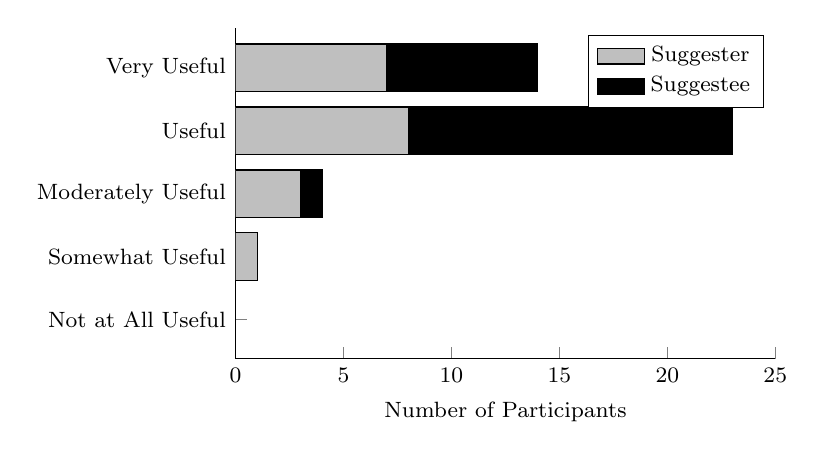
\begin{tikzpicture}
\begin{axis}[
    xbar stacked,
    ytick=data,
    axis y line*=none,
    axis x line*=bottom,
    tick label style={font=\footnotesize},
    legend style={font=\footnotesize},
    label style={font=\footnotesize},
    xtick={0,5,10,15,20,25},
    %width=.4\textwidth,
    bar width=6mm,
    xlabel= Number of Participants,
    yticklabels={Not at All Useful, Somewhat Useful, Moderately Useful, Useful, Very Useful},
    xmin=0,
    xmax=25,
    area legend,
    y=8mm,
    enlarge y limits={abs=0.625},
]
% Suggesters
\addplot[fill=lightgray] coordinates
{(0,0) (1,1) (3,2) (8,3) (7,4)};
% Suggestees
\addplot[fill=black] coordinates
{(0,0) (0,1) (1,2) (15,3) (7,4)};
\legend{Suggester, Suggestee}
\end{axis}  
\end{tikzpicture}
\caption{Survey Results on the Usefulness of \suggs}
\label{fig:sugg-usefulness}
\end{figure}


\subsection{Summary}

Our findings show that \suggs have a major influence on development practices and behavior. We discovered this feature is useful for suggesting different types of code changes, effective for facilitating recommendations during reviews, and beneficial for improving coding activity and collaboration between developers. Additionally, we found developers find \sugg useful for making and receiving recommendations on GitHub pull requests. Based on qualitative analysis examining user feedback on the advantages of \sugg, we submit two main implications for improving the future recommender systems and their developer impact. These implications include incorporating \textbf{\em user-driven communication} (\textit{Communication}, \textit{Code}, and \textit{Conciseness}) and \textbf{\em workflow integration} (\textit{Actionability}, \textit{Ease of Use}, \textit{Location}, \textit{Scalability}, and \textit{Timing}) into automated recommendations to improve developer behavior.

\section{Discussion}

To evaluate \framework, this work analyzes \suggs as a recommendation system incorporating all the principles from this conceptual framework. The findings from the evaluations of \sugg presented in this chapter show that developers prefer to receive recommendations from this system and it has a major impact on development practices on GitHub. Overall, we provide four implications for designing effective recommender systems based on the results of these studies: \textbf{\em recommendation content}, \textbf{\em recommendation design}, \textbf{\em user-driven communication}, and \textbf{\em workflow integration}. Here, we explain these conclusions from the context of each study and through the lens of the \framework framework.

\subsection{Actionability}

Our analysis of the \suggs feature suggests that actionability influences the perception and adoption of recommendations by developers. For example, the recommendation styles and developer impact study offer \textit{recommendation design} and \textit{workflow integration} as implications to improve automated suggestions from future recommender bots. To describe the impact of actionability in \sugg, I describe themes derived from qualitative feedback from developers in the studies presented in this chapter.

\subsubsection*{Workflow Details}

The recommendation styles results show that \textit{integration} details within the content of automated suggestions can influence adoption. These workflow details, describing how to install and integrate tools into development processes, also contribute to the actionability of recommendations by providing information on how easy it is to adopt tools and practices. For example, participants mentioned they were interested in learning if suggested tools would easily work with ``\textit{whatever CI or test runner system I've got}'' (P8) and wanted to know if they had ``\textit{simple integration}'' (P1). Similarly, developers desired information on the \textit{reliability} of systems to learn about their stability and how well tools do the things they claim to do.

Furthermore, participants mentioned designing automated recommendations to include relevant \textit{examples} of usage. For instance, P14 stated ``\textit{specific examples...would be a lot more compelling}'' and P10 noted ``\textit{It would be better if they can show me some examples with some very clear results like this is something you can get with our tool}''. Additionally, developers were interested in testing out the actionability of recommendations saying  ``\textit{I would like to try it by myself first}'' (P11) and ``\textit{I would test it out locally}'' (P8). By incorporating details on the actionability of recommendations this concept into developer recommendations such as how to install tools, integrate them into CI build systems, and the existence of plugins within popular IDEs, automated recommendations can increase the likelihood of adoption for developer behaviors. 


\subsubsection{Workflow Integration} 

Both \suggs studies show the importance of integrating recommendations effectively into developer workflows. For instance, developers were likely to adopt tool recommendations from \sugg over other recommender systems because of its ability to automatically apply recommendations and its ``neat integration'' (P7). Our preliminary work also shows that integration is a key factor in developer adoption, with the disruptiveness of notifications from \toolone discouraging users from adopting recommendations. However, we found developers were more likely to adopt automated static analysis tool recommendations from actionable systems such as \suggs. 

The developer impact study also found actionability increased adoption of code change suggestions. We found \sugg were more popular and more effective than static pull request review comments with fenced code. Our qualitative results also showed this was one of the most useful aspects of this recommendation system. For example, participants mentioned they found ``\textit{the ability for people to be able to suggest changes and to be able to incorporate those changes immediately}'' (\see8) and the fact suggestions can be ``\textit{accepted right away, without requiring copy pasting and committing on my side}'' (\see9) useful for receiving recommendations. Additionally, developers reported \textit{ease of use} and \textit{scalability} contributed to the ability to easily adopt \sugg into code review processes and make suggestions to developers. Hence, we show actionability can enhance automated recommendations and improve the effectiveness of recommender systems.

\subsection{Feedback}

The \sugg studies also show that the information provided to users in automated recommendations impacts adoption. For example, we found \textit{recommendation content} influences the style of automated recommendations and \textit{user-driven communication} is a favorable aspect of \suggs. To illustrate the importance of feedback in recommendations with this system, I outline themes provided by developers from the results of the recommendation styles and developer impact studies. 

\subsubsection{Relevance}

Developers in the recommendation styles study reported details concerning the relevance of tools impacts their decisions on adoption. For instance, P2 mentioned the content of recommendations helps them decide whether ``\textit{it's something I really need or want}'', P9 stated ``\textit{the recommendation itself matters less than how much I need the thing...If I don’t need it then I’m not going to try it}'', and P12 declared they ``\textit{don't really care}'' about tools that are irrelevant to their work. Participants were specifically interested in receiving information about integration details, the reputation of tools, and the trustworthiness of systems. Alternatively, irrelevant recommendations that ``\textit{show some other useless stuff which may confuse the potential user}'' (P10) can lead to ineffective recommendations. For example, we found \tele suggestions were not useful because they provided irrelevant and generic feedback in recommendations to users.

Similarly, developers expressed disdain for recommendation content that appears to be \textit{marketing} or advertisements. For example, developers described the email recommendation stating it sounds ``\textit{pretty suspicious}'', ``\textit{email...there’s so much stuff that comes through email}'' (P1), ``\textit{email is definitely a no}'' (P7), and ``\textit{I'd immediately delete it}'' (P6). Additionally, P5 mentioned ``\textit{I’m not somebody who likes to get unsolicited marketing stuff}''. The negative perception of marketing in software engineering can also be found from the backlash received by maintainers of the StandardJS JavaScript style guide, linter, and formatting tool,\footnote{\url{https://standardjs.com/}} who attempted to raise funds for development by incorporating advertisements inside the terminal.\footnote{\url{https://github.com/standard/standard/issues/1381}} In this instance, we found poor feedback in suggestions discouraged users from adopting recommendations and contend automated systems should avoid marketing language in recommendations.

However, we found details about the \textit{popularity} of systems plays a key role in adoption according to participants in the recommendation styles study. Most developers desired information the reputation of tools when making decisions, stating ``\textit{one of the things I want to see is what other people think about it}'' (P3), ``\textit{how many people use it...the popularity of the tool being used would influence me to try that}'' (P6), ``\textit{when there’s a buzz around a tool, that’s when you know it’s good and you know it’s worth checking out}'' (P12), and recommendations should ``\textit{try to highlight the popularity, popularity is so crucial}'' (P13). 

Participants also mentioned using various sources for learning about the reputation of tools, such as from peers (i.e. ``\textit{word of mouth and people that I actually trust who use it}'' (P6)) and online searches (i.e. ``\textit{Google the tool's name...[and get] a link on the first page}'' (P5)) in addition to social media and other online programming communities. Prior work also shows displaying details about popularity impact adoption of developer behaviors, such as increasing updates to repositories and contributions from collaborators~\cite{aggarwal2014co}. This indicates automated recommendations should consider incorporating popularity statistics such as number of users, downloads, social media followers, and reviews to encourage adoption. Thus, we argue including relevant feedback about tools and practices is necessary to encourage the adoption of developer behaviors

\subsubsection{Conciseness}

The recommendation styles and developer impact study found users appreciated the brief and compact nature of recommendations with \suggs. For example, when describing the email and issue static analysis tool recommendations mentioned they contained ``\textit{a ton of words}'' and were ``\textit{way too lengthy}'' (P13). Additionally, P10 noted effective recommendations ``\textit{just get[sic] to the point}''. However, P8 liked \sugg because they provide a ``\textit{nice, concrete error}'' (P8). Even though all of the recommendation styles contained similar text in the suggestion, systems such as email appeared to contain more text for developers to read. Likewise, research suggests software engineers prefer instant messaging systems because they are more concise and quicker than emails~\cite{blatt2013email}.

\textit{Concise} recommendations with \suggs also played a role in impacting developer behavior. For example, \ser11 noted ``\textit{it uses less words}''. Developers also reporting preferring recommendations as \textit{code} stating this system ``\textit{can quickly and precisely show what change they expect. Describing the change with words is pretty annoying}'' (\see12), ``\textit{removes guesswork from interpreting a prose explanation}'' (\ser4), and ``\textit{removes all ambiguity about what I'm asking for if I can just directly put the code there}'' (\ser12). Prior work also found conciseness is important designing interactive software systems~\cite{wasserman1981user} and in \textit{quick fix designs} to increase adoption of code-checking systems~\cite{Johnson2013Why}.

\subsubsection{Communication}

The developer impact study results show one of the most useful aspects of \sugg is their ability to effectively communicate to developers. Participants found this system effective for facilitating clear communication between developers on pull requests. For instance, users replied this system is useful because it ``\textit{lets someone else directly make changes instead of writing out instructions on how to make changes}'' (\see10), ``\textit{gives the suggestion in a very clear way}'' (\ser5), and provides ``\textit{easy information on what to change in your pull request}'' (\see5). This \textit{user-driven communication} led to effective recommendations from developers on pull requests. Prior work also suggests poor communication from automated systems prevents static analysis tool adoption~\cite{Johnson2013Why} and frustrates developers during interactions with bots~\cite{wessel2018power}, while \textit{user-driven conversations} improves the effectiveness of recommender chatbots~\cite{cerezo2019building} while specific and clear language can overcome barriers to security adoption adoption~\cite{Xiao2014Security}. We propose implementing clear communication focused on users to improve automated developer behavior recommendations. Overall, we conclude developers are more likely to adopt recommendations with relevant, concise, and clear feedback.


\subsection{Locality}

\suggs provide support recommendation locality because of their ability to situate suggestions on lines of code and present recommendations during code reviews. We found this \textit{recommendation design} for the placement and timing of notifications increased the likelihood of developers adopting behaviors. These related findings from our studies are presented below.

\subsubsection{Timing} For the recommendation styles user study, we found the systems with more convenient temporal locality (\suggs) were more likely to convince developers to adopt static analysis tools than those with low temporal locality (pull requests, issues, and emails). We refer to these systems as having low temporal locality because, unlike \sugg, they can appear to developers in their email or repository any time during the development process. However, \sugg are limited to open pull requests currently under review. Similarly, previous research in software engineering shows untimely recommendations prevented programmers from adopting code navigation recommendations from Spyglass~\cite{viriyakattiyaporn2009challenges} while timely notifications increased the amount of Infer\footnote{\url{https://fbinfer.com/}} and Zoncolan\footnote{\url{https://engineering.fb.com/2019/08/15/security/zoncolan/}} static analysis warnings by developers at Facebook~\cite{Distefano2019Facebook}.

In the developer impact study, many survey respondents commented on how \suggs impacted the timing of reviews. For example, developers mentioned this feature ``\textit{lets me do reviews much faster}'' (\ser3), ``\textit{accelerates getting pull requests accepted}'' (\see4), ``\textit{it's great to be able to quickly apply changes}'' (\see23), and ``\textit{it's often quicker both to suggest a minor change}'' (\ser8). Our quantitative analysis also found that, while \sugg lengthen the overall pull request review process, they are significantly faster for making recommendations and responding to suggestions during the code review process. Therefore, to design effective automated recommendations, systems should focus on making suggestions to developers at convenient times within the development workflow. 

\subsubsection{Location}

Our recommendation style study results also suggest that the placement of notifications is important for developer recommendations. For example, we found participants were least likely to adopt recommendations from emails, the system with the worst spatial locality in a separate window outside of the repository. As the spatial locality of recommendations improved, we found developers were more likely to adopt static analysis tool recommendations with \suggs, the most conveniently located notification on the line of code, being the most effective. P5 also mentioned the location of recommendations influences their decision on whether or not to adopt, noting they did not want to ``\textit{go to [the tool's] website and have to click through a million different links}''. Prior work shows tool recommendations within the coding panels of IDEs can increase efficiency and are preferred by developers~\cite{Flower} in addition to minimizing \textit{visual momentum} and helping programmers feel less disoriented in their development environment~\cite{de2006using}.

Participants in the developer impact study also praised the location of \sugg. For example, \see24 stated this feature is useful because there is ``\textit{no need to leave the pull request page to make a suggested change}''. GitHub developers also added this feature is useful because it ``\textit{shows suggested code changes integrated with the actual source}'' (\see22) and ``I can just directly put the code there'' (\ser 13). Thus, we argue automated recommendations should appear at convenient locations within the programming environment in order to increase the likelihood of adoption and improve the behavior of developers. \\

Overall, the results of the \suggs studies show that this system is preferred by developers for receiving recommendations and effective for improving development practices. This system, which incorporates the \framework framework, uses this framework to make actionable, relevant, clear, and convenient recommendations to developers. The feedback provided from developers through semi-structured interviews and surveys confirm the presence of these framework principles contribute to the effectiveness of \sugg on GitHub. Ultimately, we conclude \framework is a useful mechanism for creating automated recommendations because of its focus on recommendation content and design as well as fostering user-driven communication and facilitating workflow integration.








